\documentclass[aspectratio=169,t,13pt,usenames,dvipsnames]{beamer}
\usetheme[lily]{PaloAlto}
\usecolortheme{dolphin}
\usepackage{mathtools}
\usepackage{lmodern}
\usepackage{tikz}
\usepackage{pgfplots}
\usepackage{tikz-3dplot}
\usepackage{adjustbox}
\usetikzlibrary{quantikz}
\usepackage{xcolor}
\usepackage{bm}
\pgfplotsset{compat=newest}
\logo{%
\stackbox[c][c]{
\includegraphics[height=1.15cm]{logo.pdf}\\[-3pt]{\textcopyright~2022}\\{Ron K. Cytron}}}

% \logo{
\includegraphics[height=2.5cm]{logo.pdf}}
\def\ColorR#1{\textcolor{BrickRed}{#1}}
\def\ColorG#1{\textcolor{\RCthree}{#1}}
\def\ColorB#1{\textcolor{\RCtwo}{#1}}
\definecolor{links}{HTML}{2E8B57}
\hypersetup{colorlinks,linkcolor=,urlcolor=links}
%%
%% From stackoverflow
%%
\newcommand{\MyArrow}[1][0.1pt]{\tikz[baseline=-0.26em,y=3em, x=3em]{\filldraw[line width=#1] (0.4202,0.0021) .. controls (0.4202,-0.0000) and (0.4188,-0.0018) .. (0.4171,-0.0025) .. controls (0.3917,-0.0092) and (0.3699,-0.0236) .. (0.3509,-0.0401) .. controls (0.3355,-0.0538) and (0.3225,-0.0704) .. (0.3130,-0.0890) .. controls (0.3119,-0.0915) and (0.3094,-0.0929) .. (0.3066,-0.0929) .. controls (0.3028,-0.0929) and (0.2996,-0.0897) .. (0.2996,-0.0858) .. controls (0.2996,-0.0848) and (0.3000,-0.0837) .. (0.3003,-0.0827) .. controls (0.3087,-0.0665) and (0.3193,-0.0517) .. (0.3316,-0.0391) -- (0.1181,-0.0391) .. controls (0.1143,-0.0391) and (0.1111,-0.0359) .. (0.1111,-0.0320) .. controls (0.1111,-0.0282) and (0.1143,-0.0250) .. (0.1181,-0.0250) -- (0.3471,-0.0250) .. controls (0.3611,-0.0137) and (0.3766,-0.0046) .. (0.3935,0.0021) .. controls (0.3766,0.0088) and (0.3611,0.0179) .. (0.3471,0.0292) -- (0.1181,0.0292) .. controls (0.1143,0.0292) and (0.1111,0.0323) .. (0.1111,0.0362) .. controls (0.1111,0.0401) and (0.1143,0.0432) .. (0.1181,0.0432) -- (0.3316,0.0432) .. controls (0.3193,0.0559) and (0.3087,0.0707) .. (0.3003,0.0868) .. controls (0.3000,0.0879) and (0.2996,0.0889) .. (0.2996,0.0900) .. controls (0.2996,0.0939) and (0.3028,0.0970) .. (0.3066,0.0970) .. controls (0.3094,0.0970) and (0.3119,0.0956) .. (0.3130,0.0932) .. controls (0.3225,0.0745) and (0.3355,0.0580) .. (0.3509,0.0443) .. controls (0.3699,0.0278) and (0.3917,0.0133) .. (0.4171,0.0067) .. controls (0.4188,0.0059) and (0.4202,0.0042) .. (0.4202,0.0021) -- cycle;}}
\def\LinkArrow#1{%
\mbox{$\,$\href{#1}{\mbox{\vrule width 0pt height 0ex depth 0pt$\MyArrow[0.75pt]$}}}$\,$}
\def\WLOG{WLOG}
\def\True{\mbox{\texttt{True}}}
\def\False{\mbox{\texttt{False}}}
\def\Zero{\mbox{$0$}}
\def\One{\mbox{$1$}}
\def\Not#1{%
\ensuremath{\Overline{\ensuremath{#1}}}}
\def\Xor#1#2{\ensuremath{#1\oplus #2}}
\def\Nand#1#2{%
\ensuremath{\mbox{Nand}(#1,#2)}}
\def\And#1#2{%
\ensuremath{#1 \wedge #2}}
\def\Or#1#2{%
\ensuremath{#1 \vee #2}}
\def\Conj#1{%
\ensuremath{#1^{\star}}}
\def\Star#1{%
\Conj{#1}}
\def\EmptyString{\ensuremath{\lambda}}
\def\Mag#1{%
\ensuremath{{|\,#1\,|}}}
\def\PNorm#1#2{\ensuremath{\Mag{\kern-2pt\Mag{#1}\kern-2pt}}_{#2}}
\def\Prob#1{%
\ensuremath{\Mag{#1}^{2}}}
\def\CNOT#1#2{%
\ensuremath{\NamedGate{CNOT}(#1,#2)}}
\def\CNOTMatrix{%
\begin{pmatrix*}[r]
1 & 0 & 0 & 0 \\
0 & 1 & 0 & 0 \\
0 & 0 & 0 & 1 \\
0 & 0 & 1 & 0\end{pmatrix*}%
}
\def\CCNOT#1#2#3{%
\ensuremath{\mbox{\NamedGate{CNOT}}(#1,#2,#3)}}
\long\def\ToDo#1{\smash{\textcolor{YellowOrange}{#1}}}
\def\ApplyGate#1#2{%
\ensuremath{#1\,#2}}
\def\Inverse#1{\ensuremath{{#1}^{-1}}}
\def\Quote#1{``#1''}
\def\NamedGate#1{%
\mbox{\bfseries{\textrm{#1}}}}
\def\Identity{\NamedGate{I}}
\def\Hadamard{\NamedGate{H}}
\def\PauliX{\NamedGate{X}}
\def\PauliY{\NamedGate{Y}}
\def\PauliZ{\NamedGate{Z}}
\def\SQBG#1#2#3#4#5{%
\ensuremath{%
#1 \begin{pmatrix*}[r] #2 & #3 \\ #4 & #5\end{pmatrix*}}}
\def\HMatrix{%
\SQBG{\RootTwo{}}{1}{1}{1}{-1}}
\def\XMatrix{%
\SQBG{\relax}{0}{1}{1}{0}}
\def\ZMatrix{%
\SQBG{\relax}{1}{0}{0}{-1}}
\def\YMatrix{%
\SQBG{\relax}{0}{-i}{i}{0}}
\def\IMatrix{%
\SQBG{\relax}{1}{0}{0}{1}}
\def\Co#1{\mathbb{C}}
\def\Implies#1#2{\ensuremath{#1 \rightarrow\ #2}}
\def\Domain#1{\ensuremath{\mathcal{#1}}}
\def\CompClass#1{\Domain{#1}}
\def\SpecialX#1{\ensuremath{#1^{\star}}}
\def\Forall#1#2{\ensuremath{\forall\ #1, #2}}
\def\Degrees#1{\ensuremath{#1^{\circ}}}
\def\RootTwo{\ensuremath{\frac{1}{\sqrt{2}}}}
\def\TwoSupOp#1#2#3{%
\ensuremath{\RootTwo{}\left(#1 #3 #2\right)}}
\def\TwoSup#1#2{%
   \TwoSupOp{\ket{#1}}{\ket{#2}}{+}}
\def\QPlus{\TwoSupOp{\QZero}{\QOne}{+}}
\def\QMinus{\TwoSupOp{\QZero}{\QOne}{-}}
\def\Set#1{\ensuremath{\left\{\,#1\,\right\}}}
\def\BigSkip{%

\bigskip

}

\def\MedSkip{%

\medskip

}
\def\SmallSkip{%

\smallskip

}
\def\SineWave#1{%
{%
\pgfmathsetmacro{\Xone}{#1}
\pgfmathsetmacro{\Xtwo}{-(#1)}
\draw (0,0) sin(1,\Xone) cos (2,0) sin(3,\Xtwo) cos (4,0);
}
}
\newcommand{\tolstrut}{%
  \vrule height\dimexpr\fontcharht\font`\A+.1ex\relax width 0pt\relax
}

\DeclareRobustCommand{\Overline}[1]{%
  \ensuremath{\overline{\raisebox{0pt}[1.07\height]{#1}}}%
}
\newenvironment{TIKZP}[1][scale=1.0]{%
\adjustbox{valign=t}\bgroup
\begin{tikzpicture}[#1]
}{%
\end{tikzpicture}
\egroup
}
\long\def\Definition#1{%
\begin{block}{Definition}
#1
\end{block}}
\long\def\Postulate#1#2{%
\begin{block}{Postulate}
\begin{description} \item[#1] #2\end{description}
\end{block}}
\long\def\TwoUnequalColumns#1#2#3#4{%
\begin{columns}%
\begin{column}{#1}#3\end{column}%
\begin{column}{#2}#4\end{column}%
\end{columns}%
}
\long\def\ThreeUnequalColumns#1#2#3#4#5#6{%
\begin{columns}%
\begin{column}{#1}#4\end{column}%
\begin{column}{#2}#5\end{column}%
\begin{column}{#3}#6\end{column}%
\end{columns}%
}
\long\def\ThreeColumns#1#2#3{%
\ThreeUnequalColumns{0.33\textwidth}{0.33\textwidth}{0.33\textwidth}{#1}{#2}{#3}%
}
\long\def\TwoColumns#1#2{%
\TwoUnequalColumns{0.5\textwidth}{0.5\textwidth}{#1}{#2}%
}
\long\def\OnlyRemark#1#2{%
\only<#1>{\Remark{#2}}}

\long\def\Remark#1{%
\begin{block}{Remark}
#1
\end{block}}
\long\def\Example#1{%
\begin{example} #1\end{example}}
\def\VV{\textit{vice versa}}
\def\QZero{\ket{\hbox to 0.7em{\hss \ensuremath{0}\hss}}}
\def\QOne{\ket{\hbox to 0.7em{\hss \ensuremath{1}\hss}}}
\def\QState#1{\ket{\QName{#1}}}
\def\QName#1{\ensuremath{\psi_{#1}}}
\def\TensOp{\ensuremath{\bm{\otimes}}}
\def\TensProd#1#2{\ensuremath{#1 \TensOp{} #2}}
\def\TensSupProd#1#2{\ensuremath{#1^{\bm{\otimes} #2}}}
\def\PZero{\SQB{1}{0}}
\def\POne{\SQB{0}{1}}
\def\PPlus{\ensuremath{\RootTwo{}\SQB{1}{1}}}
\def\PMinus{\ensuremath{\RootTwo{}\SQB{1}{-1}}}
\def\PHad{\ensuremath\frac{1}{\sqrt{2}}\SQB{1}{1}}
\def\PHadm{\ensuremath\frac{1}{\sqrt{2}}\SQB{1}{-1}}
\def\Intersect#1#2{\ensuremath{#1 \cap #2}}
\def\Union#1#2{\ensuremath{#1 \cup #2}}
\def\Set#1{\ensuremath{\left\{\,#1\,\right\}}}
\def\BinAlph#1{\ensuremath{\Set{0,1}^{#1}}}
\def\AllBits#1#2{\ensuremath{#1\in \BinAlph{#2}}}
\def\DQB#1#2#3#4{%
\ensuremath{\begin{pmatrix*}[r] #1 \\ #2 \\ #3 \\ #4\end{pmatrix*}}}
\def\QQB#1#2#3#4#5#6#7#8{%
\ensuremath{\begin{pmatrix*}[r] #1 \\ #2 \\ #3 \\ #4 \\ #5 \\ #6 \\ #7 \\ #8\end{pmatrix*}}}
\def\SQB#1#2{%
\ensuremath{\begin{pmatrix*}[r] #1 \\ #2\end{pmatrix*}}}
\def\CQB#1#2{%
\ensuremath{\begin{pmatrix*}[r] #1 #2\end{pmatrix*}}}
\def\CDQB#1#2#3#4{%
\ensuremath{\begin{pmatrix*}[r] #1 #2 #3 #4\end{pmatrix*}}}
\def\TZPointDiam{2pt}
\def\TZPoint#1#2#3{%
\draw[fill=black] (#1) circle (\TZPointDiam) node[#3] {#2} ;}
\def\UnitComplexCircle{%
\draw [<->] (-1.5, 0) -- (1.5, 0)  node[right] {$\Re{}$} ;
   \draw [<->] (0,-1.5) -- (0, 1.5) node[above] {$\Im{}$} ;

   \draw (0, 0) circle (1) ;
   }
   \def\TZPEast{\TZPoint{1,0}{$+1$}{above right}}
   \def\TZPNorth{\TZPoint{0,1}{$\NiceI{}$}{above right}}
   \def\TZPWest{\TZPoint{-1,0}{$-1$}{above left}}
   \def\TZPSouth{\TZPoint{0,-1}{$-\NiceI{}$}{below right}}
\def\TZText#1#2#3{%
  \draw (#1) node [#3] {#2};
}
\def\Qiskit{\texttt{qiskit}}
\def\TwoToThe#1{\ensuremath{2^{#1}}}
\def\Exp#1{\ensuremath{e^{#1}}}
\def\NiceI{\kern 0.5pt\ensuremath{\mathfrak{i}}}
\def\ExpPhase#1{\Exp{\,\NiceI\,#1}}
\def\ExpNegPhase#1{\Exp{-\NiceI\,#1}}
%%
%% Not sure this is used
%%
\def\PhaseLabel#1{\phase{\fbox{#1}}}
%%
\def\ColHead#1{\begin{center}\bf #1\end{center}}
\def\Complex#1#2{\ComplexGen{#1}{#2}{+}}
\def\ComplexDiff#1#2{\ComplexGen{#1}{#2}{-}}
\def\ImaginaryM#1{\ComplexDiff{\relax}{#1}}
\def\ComplexGen#1#2#3{%
\ensuremath{#1 #3 i\relax #2}}
\def\Polar#1#2{\ensuremath{#1\hbox to 0.1pt{\hss}\Exp{\NiceI\relax#2}}}
%%
%% #1 -- lower left x
%% #2 -- lower left y
%% #3 -- upper right x
%% #4 -- upper right y
%% #5 -- num lines
\def\PFilter#1#2#3#4#5{

    \draw (#1,#2) -- (#3,#2) -- (#3,#4) -- (#1,#4) -- cycle;
    \foreach \i in {1,...,#5}
    {
        \pgfmathsetmacro{\PFilterInc}{#1 + (#3-#1) / #5 * \i}
        % \edef\PFilterInc{\pgfmathresult}
        \draw (\PFilterInc, #2) -- (\PFilterInc, #4);
    }
}
%% #1 - x
%% #2 - y
%% #3 - degrees
%% #4 - options
%% #5 - radius
\def\RadiantArrowsR#1#2#3{%
\foreach \p in {0, #1,...,360} {
   \draw[#2] (0,0)  -- (\p:#3) ;
}
}
\def\RadiantArrows#1#2{%
   \RadiantArrowsR{#1}{#2}{1}
}
\newcommand\RotateTheta[1][scale=1.0]{%
\SquareOutline{}
\begin{scope}[#1]
\fill[white] (0.5,0.5) circle (0.5);
\draw (0.5,0.5) circle (0.5);
\draw[->] (1.0,0.5) arc(0:45:0.5);
\draw (0.5,0.5) node {$\theta$};
\end{scope}
}
\def\SquareOutline{%
\path (0,0) rectangle (1,1);%
}%
\newcommand\Qif[1][scale=1.0]{%
\begin{scope}[#1]
\SquareOutline{}
\clip (0,0) rectangle(1,1);
\RotateAroundCenter{45}{%
\begin{scope}
\draw (0.15,0.15) rectangle(0.85,0.85);
\end{scope}}
\end{scope}
}
\newcommand\LightSource[1][scale=1.0]{%
\begin{scope}[#1]
\SquareOutline{}
\PhotonGun{}
\begin{scope}[shift={(0.75,0.5)}]
    \RadiantArrowsR{22.5}{color=red}{0.25}
\end{scope}
\end{scope}
}
\def\PhotonGun{%
\fill (0,0.375) rectangle (0.5, 0.625);
}
\def\HPolar{%
\begin{scope}[color=red]
\SquareOutline{}
\draw[thick] (0.5,0.4) -- ++(0.35,0)
             ++(-0.35,0.1) -- ++(0.35,0)
             ++(-0.35,0.1) -- ++(0.35,0);
% \fill (0.90,0.5) circle (0.05);
\end{scope}
}
\def\VPolar{%
\begin{scope}[color=red]
\draw[thick] (0.6,0.375) -- ++(0,.250)
             ++(0.1,-.250) -- ++(0,.250)
             ++(0.1,-.250) -- ++(0,.250);
% \fill (0.95,0.5) circle (0.05);
\end{scope}
}
\newcommand\HPolarizedLightSource[1][scale=1.0]{%
\begin{scope}[#1]
\SquareOutline{}
\PhotonGun{}
\HPolar{}
\end{scope}
}
\newcommand\VPolarizedLightSource[1][scale=1.0]{%
\begin{scope}[#1]
\SquareOutline{}
\PhotonGun{}
\VPolar{}
\end{scope}
}
\newcommand\EVBomb[1][scale=1.0]{%
\begin{scope}[#1]
\fill (0.5,0.5) circle(0.5);
\end{scope}%
}
\newcommand\EVBoom[1][scale=1.0]{%
\begin{scope}[#1]
\fill[white] (0.5,0.5) circle(0.5);
\draw[red,thick] (0.5,0.5) circle(0.5);
\clip (0,0) rectangle(1,1);
\begin{scope}
\node[scale=0.35,xshift=28pt,yshift=28pt,starburst,draw,red,fill=orange,line width=1.5pt]
{BOOM!};
\end{scope}
\end{scope}
}
\newcommand\Measurement[1][scale=1.0]{%
\begin{scope}[#1]
\draw[color=white] (0,0) rectangle(1,1);
\begin{scope}
\clip (0.25,0.25) rectangle (1,1);
\draw (0,0) circle(0.9);
\draw (0,0) circle(1.0);
\end{scope}
\draw[thick] (0,0) --(0,1);
\draw[->] (0.25,0.25) -- (0.9,0.9);
\end{scope}
}
\def\TRectangle#1#2#3#4#5#6{%
\begin{scope}[#6]
\draw [fill=#5] (#1,#2) rectangle (#3,#4);
\end{scope}
}
%% #1 -- llx
%% #2 -- lly
%% #3 -- urx
%% #4 -- ury
%% #5 -- angle
\newcommand\Mirror[1][rotate=0]{%
\clip (0,0) rectangle(1,1);
\begin{scope}[#1]
   \SquareOutline{}
   \TRectangle{0}{.4375}{1}{.5625}{Gray}{rotate=0}
\end{scope}
}
\newcommand\BeamSplitter[1][scale=1.0]{%
\begin{scope}[#1]
    \SquareOutline{}
    \TRectangle{0}{.375}{1}{.625}{SkyBlue}{rotate=0}
\end{scope}
}
\def\MZ{%
\LightSource{}
\Shift{2}{0}{\RotateAroundCenter{-45}{\BeamSplitter{}}}
\Shift{2}{-2}{\RotateAroundCenter{-45}{\Mirror{}}}
\Shift{6}{0}{\RotateAroundCenter{-45}{\Mirror{}}}
\Shift{6}{-2}{\RotateAroundCenter{-45}{\BeamSplitter{}}}
\Shift{8}{-2}{\Measurement[color=orange]{}}
\Shift{6}{-4}{\RotateAroundCenter{-90}{\Measurement[color=\RCtwo]{}}}
}
\def\Shift#1#2#3{%
\begin{scope}[shift={(#1,#2)}] #3\end{scope}
}
\def\RotateAroundCenter#1#2{%
\begin{scope}[rotate around={#1:(0.5,0.5)}]
  #2
\end{scope}
}
\def\Vskip#1{\mbox{}\vskip #1\mbox{}}
\def\Hskip#1{\mbox{}\hskip #1\mbox{}}
\author{Ron K.~Cytron}
\institute{Washington University\\Saint Louis, Missouri\\[2em] \textcopyright~2022 All rights reserved by the author}
\setbeamertemplate{footline}[frame number]{}
%\setbeamertemplate{footline}[text line]{%
%  \parbox{\linewidth}{\vspace*{-8pt}\textcopyright~2021\hfill\insertshortauthor\hfill\insertpagenumber}}
%% #1 -- lecture number
%% #2 -- lecture title
%% #3 -- lecture subtitle
%% #4 -- lecture label
\def\SetTitle#1#2#3#4{%
   \title{#2}%
   \subtitle{#3}%
   \date{\today}%
   %\begin{frame}\maketitle\end{frame}%
   \frame{\titlepage}%
   \lecture[#1]{#2: #3}{lec:#4}%
}
\def\Kaye{\href{https://dl.acm.org/doi/10.5555/1206629}{Kaye}}
\def\MikeIke{\href{https://dl.acm.org/doi/10.5555/1972505}{Nielson~and~Chuang}}

\newcounter{ProtocolDialogStep}
\newenvironment{ProtocolDialog}[3]{%
\def\Incr{\stepcounter{ProtocolDialogStep}}
\def\Ref##1{\Incr{}\ThreeUnequalColumns{#1}{#2}{#3}{\arabic{ProtocolDialogStep}. ##1}{\relax}{\relax}}%
\def\Alice##1{\Incr{}\ThreeUnequalColumns{#1}{#2}{#3}{\relax}{\arabic{ProtocolDialogStep}. ##1}{\relax}}%
\def\All##1##2##3{%
\Incr{}
\ThreeUnequalColumns{#1}{#2}{#3}{\arabic{ProtocolDialogStep}. ##1}{##2}{##3}
}
\def\Bob##1{\Incr{}\ThreeUnequalColumns{#1}{#2}{#3}{\relax}{\relax}{
\arabic{ProtocolDialogStep}. ##1}}%
\setcounter{ProtocolDialogStep}{0}%
\ThreeUnequalColumns{#1}{#2}{#3}{\textbf{Ref}}{\textbf{Alice}}{\textbf{Bob}}
}{%
}
%% #1 -- options
%% #2 -- width
%% #3 -- height
%% #4 -- signals
\newenvironment{GateBox}[4][scale=1.0]{%
\edef\Signals{#4}%
\edef\Height{#3}%
\edef\Width{#2}%
\pgfmathsetmacro{\Max}{\Signals}%
\pgfmathsetmacro{\Vsep}{\Height / \Max}%
\pgfmathsetmacro{\Wlen}{\Width / 5}%
\def\ComputeMyY##1{%
   \pgfmathsetmacro{\MyY}{\Height - 0.5 * \Vsep - ##1*\Vsep}}%
\def\Input##1##2{%
   \pgfmathsetmacro{\Xone}{-\Wlen}
   \pgfmathsetmacro{\Xtwo}{0}
   \pgfmathsetmacro{\MyY}{\Height - 0.5 * \Vsep - ##1*\Vsep}
   \draw[->] (\Xone,\MyY) node[left] {##2} -- (\Xtwo,\MyY);
}%
\def\Output##1##2{%
   \pgfmathsetmacro{\Xone}{\Width}
   \pgfmathsetmacro{\Xtwo}{\Width + \Wlen}
   \pgfmathsetmacro{\MyY}{\Height - 0.5 * \Vsep - ##1*\Vsep}
   \draw[->] (\Xone,\MyY) -- (\Xtwo,\MyY) node[right] {##2};
}%
\def\BoxLabel##1{%
\node[draw, fit={(0,0) (\Width,\Height)}, inner sep=0pt, label=center:\mbox{##1}] (A) {};
}%
\begin{TIKZP}[#1]
   \draw (0,0) rectangle(#2,#3);
}{%
\end{TIKZP}}
%%
%% 1 options
%% 2 width
%% 3 height
%% 4 number of qubits
%%
\newenvironment{DotPBox}[4][scale=1.0]{%
\edef\Qubits{#4}%
\edef\Height{#3}%
\edef\Width{#2}%
\pgfmathsetmacro{\Max}{\Qubits}%
\pgfmathsetmacro{\Hsep}{\Width / \Max}%
\def\Qbit##1##2{%
   \pgfmathsetmacro{\MyX}{##1*\Hsep}
   \draw (\MyX,0) rectangle ++(\Hsep,\Height) node[pos=0.5] {\ensuremath{##2}};
}%
\begin{TIKZP}[#1]
}{%
\end{TIKZP}}
\def\PhiTheta#1#2{%
\mbox{\ensuremath{\textcolor{\RCone}{\phi = #1}, \textcolor{\RCtwo}{\theta = #2}}}}
%
% #2 -- orcacle name
% #3 -- upper left input
% #4 -- lower left input
% #5 -- upper right output
% #6 -- lower right output
%
\newenvironment{Oracle}[6][scale=1.0]{%
\begin{GateBox}[#1]{2.5}{1.5}{2}
\BoxLabel{#2}
\Input{0}{#3}
\Input{1}{#4}
\Output{0}{#5}
\Output{1}{#6}
}{%
\end{GateBox}
}
\newenvironment{TTable}[3]{%
\def\TRow##1##2##3{%
##1 & ##2 & ##3 \\}
\begin{tabular}{c|cc}
\TRow{#1}{#2}{#3}\hline
}{%
\end{tabular}
}
%%
%%  1 name
%%  2 one x
%%  3 one f(x)
%%  4 another x
%%  5 another f(x)
\def\SBitTable#1#2#3#4#5{%
\begin{center}
    \begin{TTable}{#1}{$x$}{$f(x)$}
    \TRow{ }{#2}{#3}
    \TRow{ }{#4}{#5}
    \end{TTable}
\end{center}}
%%
%%
\newenvironment{UTable}[6]{%
\def\URow##1##2##3##4##5##6{%
##1 & ##2 & ##3  & ##4 & ##5 & ##6\\}
\begin{tabular}{c|cc|c|cc}
& \multicolumn{2}{|c|}{Inputs} &
& \multicolumn{2}{|c}{Outputs} \\
\URow{#1}{#2}{#3}{#4}{#5}{#6}\hline
}{%
\end{tabular}
}
%%
%%  1 name
%%  2 one x
%%  3 one f(x)
%%  4 another x
%%  5 another f(x)
\def\SBitTable#1#2#3#4#5{%
\begin{center}
    \begin{TTable}{#1}{$x$}{$f(x)$}
    \TRow{ }{#2}{#3}
    \TRow{ }{#4}{#5}
    \end{TTable}
\end{center}}

\newenvironment{BlochSphere}[3][scale=1.0]{
    \bgroup%
    \def\BlochSpherePhiTheta{%
    \tdplotsetrotatedcoords{0}{0}{0};O
        \path[tdplot_rotated_coords] (1.0,0,0) arc (0:115:1.0) node(phi) {};
        \draw[tdplot_rotated_coords,thick,\RCone] (0.3,0,0) arc (0:115:0.3);
        \draw[tdplot_rotated_coords,\RCone,thick,dashed] (0,0,0) -- (phi);
        \draw[\RCone] (0.4,0.4,0) node {$\phi$};
        
        \tdplotsetrotatedcoords{25}{-90}{0};
        \path[tdplot_rotated_coords] (1,0,0) arc (0:45:1) node(theta) {};
        \draw[tdplot_rotated_coords,thick,\RCtwo] (0.4,0,0) arc (0:45:0.4);
        \draw[tdplot_rotated_coords,\RCtwo,thick] (0,0,0) -- (theta);
        \draw[\RCtwo] (-0.4,0,0.3) node {$\theta$};
        
        
    }
    \def\TZPointDiam{0.7pt}%
    \def\ShowAxes{%
    \draw[dashed, tdplot_rotated_coords, black] (1,0,0) node {{\Large\bf x}} (0,1,0) node {{\Large\bf y}} (0,0,1) node {{\Large\bf z}};
    }%
    \tdplotsetmaincoords{#2}{#3}%
    \begin{tikzpicture}[tdplot_main_coords, #1]
        
        
        \shade[ball color = lightgray, opacity = 0.5] (0,0,0) circle (1cm);
        
        %%
        %% The equator
        %%
        \tdplotsetrotatedcoords{0}{0}{0};
        \draw[dashed, tdplot_rotated_coords, gray] (0,0,0) circle (1);
        
        %%
        %% Arc in the x-z plane
        %%
        \tdplotsetrotatedcoords{90}{90}{90};
        \draw[dashed, tdplot_rotated_coords, gray] (1,0,0) arc (0:180:1);
        
        %%
        %% Arc in the y-z plane
        %%
        \tdplotsetrotatedcoords{0}{90}{90};
        \draw[dashed, tdplot_rotated_coords, gray] (1,0,0) arc (0:180:1);
        
        %\tdplotsetrotatedcoords{90}{90}{90};
       % \draw[dashed, tdplot_rotated_coords, black] (1,0,0) node {{\Large\bf x}} (0,1,0) node {{\Large\bf y}} (0,0,1) node {{\Large\bf z}}; 
        
        \draw[dashed, gray] (0,0,0) -- (-1,0,0);
        \draw[dashed, gray] (0,0,0) -- (0,-1,0);
        \draw[dashed, gray] (0,0,0) -- (0,0,-1);
        
        \draw[-stealth] (0,0,0) -- (1.30,0,0);
        \draw (1.45,0,0) node {$x$};
        \draw[-stealth] (0,0,0) -- (0,1.30,0);
        \draw(0,1.45,0) node {$y$};
        \draw[-stealth] (0,0,0) -- (0,0,1.30);
        \draw (0,0,1.45) node {$z$};
        
}{%
    \end{tikzpicture}
    \tdplotsetmaincoords{0}{0}
    \egroup
}

\long\def\Exercise#1#2{%
\relax}
\newcommand\QEDsym[1][2em]{\hbox to #1{\hss\ensuremath{\square}}}
\def\QED{\begin{flushright}\ensuremath{\square}\end{flushright}}
\def\UGateA{%
\ensuremath{\cos(\theta/2)}}
\def\UGateB{%
\ensuremath{-\ExpPhase{\lambda}\sin(\theta/2)}}
\def\UGateC{%
\ensuremath{\ExpPhase{\phi}\sin(\theta/2)}}
\def\UGateD{%
\ensuremath{\ExpPhase{(\phi+\lambda)}\cos(\theta/2)}}
\def\UGate{%
\SQBG{\relax}{\UGateA{}}{\UGateB{}}{\UGateC{}}{\UGateD{}}}%
\def\FCirc#1{%
\begin{tikzpicture}[scale=#1]%
\SquareOutline{}%
\fill (0.5,0.5) circle(0.4);%
\end{tikzpicture}%
}%
\def\SCirc{\FCirc{0.3}}%
\newenvironment{BBKey}[0]{%
\def\STD{%

\begin{tikzpicture}[scale=0.35]%
\SquareOutline{}%
\draw[ultra thick,purple] (0,0.5) -- (1,0.5);%
\draw[ultra thick,purple] (0.5,0) -- (0.5,1);%
\end{tikzpicture}}%
\def\HDM{%

\begin{tikzpicture}[scale=0.30]%
\SquareOutline{}%
\draw[ultra thick,purple] (0,0) -- (1,1);%
\draw[ultra thick,purple] (0,1) -- (1,0);%
\end{tikzpicture}}%
\def\BBUp{%

\begin{tikzpicture}[scale=0.30]%
\SquareOutline{}%
\draw[->,thick,purple] (0.5,0) -- (0.5,1);%
\end{tikzpicture}}%
\def\BBRt{%

\begin{tikzpicture}[scale=0.30]%
\SquareOutline{}%
\draw[->,thick,purple] (0,0.5) -- (1,0.5);%
\end{tikzpicture}}%
\def\BBNe{%

\begin{tikzpicture}[scale=0.30]%
\SquareOutline{}%
\draw[->,thick,purple] (0,0) -- (1,1);%
\end{tikzpicture}}%
\def\BBSe{%

\begin{tikzpicture}[scale=0.30]%
\SquareOutline{}%
\draw[->,thick,purple] (0,1) -- (1,0);%
\end{tikzpicture}}%
\def\BBBasis{%
\begin{tabular}{c|c|c}
Basis & 0 & 1 \\
\hline
\STD{} & \BBUp{} & \BBRt{} \\
\HDM{} & \BBNe{} & \BBSe{}
\end{tabular}%
}%
}{%
\relax%
}
\def\CFCirc#1{%
  \textcolor{#1}{\FCirc{0.30}}}
\def\Agree{%
  \textcolor{green}{\FCirc{0.30}}}%
\def\DisAgree{%
   \textcolor{red}{\FCirc{0.30}}}%
\def\MetaAgree{%
   \textcolor{yellow}{\FCirc{0.30}}}%
\newenvironment{EKey}[0]{%
\def\ZZ{%
\ZRot{0}%
}%
\def\ZZPO##1{%
\ZRot{\frac{\pi}{##1}}%
}%
\def\ZZNPO##1{%
\ZRot{\ensuremath{\,-\frac{\pi}{##1}}}%
}%
\def\ZRot##1{%
\ensuremath{Z_{##1}}%
}%
}{%
}
\def\AltAlert#1#2#3{%
\alt<#1>{\alert{#2}}{#3}}
\def\RCone{Rhodamine}
\def\RCtwo{CornflowerBlue}
\def\RCthree{LimeGreen}
\def\RCfour{Tan}
\def\RCfive{Plum}
\def\ColorOne#1{\textcolor{\RCone}{#1}}
\def\ColorTwo#1{\textcolor{\RCtwo}{#1}}
\def\ColorThree#1{\textcolor{\RCthree}{#1}}
\def\ColorFour#1{\textcolor{\RCfour}{#1}}
\def\ColorFive#1{\textcolor{\RCfive}{#1}}
\def\ColorBlack#1{\textcolor{black}{#1}}
\def\NegF#1{\NegOneExp{f(#1)}}
\def\NegOneExp#1{\ensuremath{(-1)^{#1}}}
\def\RootTwoN#1{\ensuremath{\frac{1}{\sqrt{2^{#1}}}}}
%%
%% var, exponent
%%
\def\SumBV#1#2{\OpBV{#1}{#2}{\displaystyle\sum\limits}}
\def\OpBV#1#2#3{\ensuremath{#3_{\AllBits{#1}{#2}}}}
\def\DotP#1#2{\ensuremath{#1\boldsymbol{\cdot}#2}}
\def\SumPH#1#2{\displaystyle\sum\limits_{#1=0}^{2^{#2}-1}}
%
% for hadamard results
%
%% #1 w for H((w>)
%% #2 free variable name
%% #3 n
\newcounter{HTableCounter}
\newenvironment{HTable}[3]{%
%% ##1 v^w
%% ##2 v . w
%% ##3 result
%% ##4 basis vector 000 001 etc.
\def\TE##1##2##3##4{%
\ensuremath{##4} & \ensuremath{##1} & \ensuremath{##2} & \ensuremath{##3 1} \ensuremath{\ket{##4}}}%
\begin{tabular}{c|c|c|r}
\multicolumn{4}{c}{$\sqrt{2^{#3}}$\,\Hadamard(\ket{#1})} \\ 
$v$ & \And{v}{#1} & \DotP{v}{#1} &  \multicolumn{1}{|c}{Term} \\ \hline}{%
\end{tabular}
}

\newcounter{ScrollCounter}
\newcounter{ScrollCounterEnd}
\newcounter{ScrollEOne}
\newcounter{ScrollETwo}
\newcounter{ScrollEThree}
\newcounter{ScrollEFour}
%%
%% start
%%
\newenvironment{ScrollingProof}[1][1]{%
   \setcounter{ScrollCounter}{#1}%
   \setcounter{ScrollEOne}{#1}%
   \setcounter{ScrollETwo}{#1}%
      \stepcounter{ScrollETwo}%
   \setcounter{ScrollEThree}{#1}%
      \stepcounter{ScrollEThree}\stepcounter{ScrollEThree}%
   \setcounter{ScrollEFour}{#1}%
      \stepcounter{ScrollEFour}\stepcounter{ScrollEFour}\stepcounter{ScrollEFour}
   \def\Curr{\value{ScrollCounter}}%
   \def\One{\value{ScrollEOne}}%
   \def\Two{\value{ScrollETwo}}%
   \def\Three{\value{ScrollEThree}}%
   \def\Four{\value{ScrollEFour}}%
   %\def\Memo##1{\gdef\RCScrollMemoText{##1}##1}
   %\def\Recall{\RCScrollMemoText}
   \def\Next##1##2{%
       \visible<\value{ScrollCounter}-##1>{##2}%
       %\def\Last{##2}%
    \stepcounter{ScrollCounter}%
    \stepcounter{ScrollEOne}%
    \stepcounter{ScrollETwo}%
    \stepcounter{ScrollEThree}%
    }%
    \def\Last##1{%
        \gdef\ScrollingLastText{##1}%
        \Next{\Two}{\visible<\value{ScrollETwo}>{\alert{\ensuremath{\big\Uparrow}}\ }##1}}%
}{%
}
\long\def\ScrollProof#1#2#3{%
\only<#1-#2>{%
\begin{ScrollingProof}[#1]
\begin{align*}
#3
\end{align*}
\end{ScrollingProof}}}
\def\RVDots{\raisebox{0.5em}{\ensuremath{\vdots}}}
%%
%% #1 -- the state undergoing hadamard
%% #2 -- the number of bits
%% #3 -- the free variable
\def\NHadamard#1#2#3{%
\SumBV{#3}{#2} \NegOneExp{\DotP{#1}{#3}} \ket{#3}}
\newenvironment{Reasoning}{%
\def\Reason##1##2{%
   \only<##1>{\makebox(0,0)[l]{\alert<##1>{\textit{##2}}}}}%
%%
%% #1 -- the range for overlays
%% #2 -- the color
%% #3 -- x
%% #4 -- y
%% #5 -- width
%% #6 -- height
%%
\def\CallOut##1##2##3##4##5##6{%
    \Reason{##1}{\Highlight{##2}{##3}{##4}{##5}{##6}}}
\vrule width 0pt depth 0.5em height 0.5em}{%
}
\def\Span#1{\ensuremath{{\mbox{span}(#1)}}}
\def\EmptySet{\Set{\,}}
%%
%% Large Binary Point
%%
\def\LBP{\mbox{\Huge .\hskip -1pt}}
%%
%% #1 color
%% #2 x loc
%% #3 y loc
%% #4 width
%% #5 height
\def\Highlight#1#2#3#4#5{%
\begin{tikzpicture}[overlay]
\draw[fill=#1,opacity=0.2] (#2,#3) rectangle ++(#4,#5);
\end{tikzpicture}}
\def\Indent#1{\mbox{}\hbox to #1{\hss}}
\newenvironment{ReverseDiag}[1][scale=1.0]{%
%%
%% ##1 color
%% ##2 location
%%
\def\BallRadius{0.45}
\def\BBall##1##2{\fill[##1,fill opacity=0.7] ##2 circle(\BallRadius);}
\begin{TIKZP}[#1]
    \draw[thick,draw=black,fill=gray, fill opacity=0.2] (0,0) -- ++(2,0) -- ++(0.5,-0.5) -- ++(0,-3) -- ++(-2.0,0) -- ++(-0.5,0.5) -- cycle;
    \draw[thick,draw=black,fill=gray] (0.5,0) -- ++(0,1)  -- node[above right,pos=0.5] {1-in} ++(1,0) -- ++(0,-1) -- cycle;
    \draw[thick,draw=black,fill=gray] (0,-0.7) -- ++(-1,0)  -- node[below left] {0-in} ++(0,-1) -- ++(1,0) -- cycle;
    \draw[thick,draw=black,fill=gray] (0.5,-3.5) -- ++(0,-1) -- ++(1.5,0) node[below right,pos=0.5] {1-out} -- ++(0,1) -- cycle;
    \draw[thick,draw=black,fill=gray] (2.5,-0.7) -- ++(1,0) -- ++(-0,-0.9) node[right] {0-out}-- ++ (-1,0) -- cycle;
    \draw[thick,draw=black,fill=\RCfour] (2.5,-1.75) -- ++(1,0) -- ++(-0,-1) node[right] {AND-out}-- ++ (-1,0) -- cycle;

}{%
\end{TIKZP}
}
\newenvironment{Pixture}[3][width=1.0\textwidth]{%
\begin{TIKZP}
\node at (0,0)
    {\includegraphics[#1]{#2/#3}}; 
}{%
\end{TIKZP}
}


% \AtBeginLecture{\frame{\Large \insertlecture}}
%%
%% test
%%
\begin{document}
\SetTitle{5}{Introduction to quantum systems}{How do we represent a quantum system?}{05}

\section{Overview}

\begin{frame}{Overview}{What will we study here?}
\begin{itemize}
    \item We characterize the state of a quantum system.
    \item Each state is a unit vector of complex numbers, one for each possible measurement outcome of the system.
    \item Each complex number is a \emph{wave amplitude}, which determines
    \begin{itemize}
        \item the probability of measuring the associated outcome
        \item how the state is affected by quantum gates
    \end{itemize}
    \item We initially investigate these ideas using photons and optical components.
    \item The \href{https://lab.quantumflytrap.com/lab}{quantum games} website is a useful and fun way to explore these ideas.
    \begin{itemize}
        \item A simpler antecedent of that website is \href{http://play.quantumgame.io/}{here}.
    \end{itemize}
    
    
\end{itemize}
    
\end{frame}

\begin{frame}{Orthogonality}{A set of mutually exclusive outcomes}
\begin{itemize}
    \item A quantum computing system contains elements, such as electrons, ions, or photons, whose quantum behavior can be influenced to achieve computation.
    \item When measured, each quantum element will be in one of a mutually orthogonal set of $d$~states.
    
\end{itemize}
\OnlyRemark{2}{In a physical system, the outcomes will be physically exclusive, so that only one of the~$d$ outcomes can ever occur.

Mathematically, we will model that behavior using orthogonal basis vectors.}
\end{frame}

\section{Quantum games}

\begin{frame}{Quantum game components}{From \href{http://play.quantumgame.io/}{Play Quantum games}}

\TwoUnequalColumns{0.65\textwidth}{0.35\textwidth}{%

\begin{itemize}

    \item<1-> The ideal light source emits exactly one photon at a time.  We are interested in the path(s) a single photon can take.
    \item<2-> The mirror reflects a photon at a \Degrees{90} angle.
    \item<3-> With equal probability, \alert<3>{yet utter unpredictability}, the beam splitter takes a photon and either
    \begin{itemize} 
       \item allows the photon to continue undisturbed, or
       \item reflects the photon like a mirror \alert<3>{($+$ more)}.
    \end{itemize}
\end{itemize}

}{%
\Vskip{-3em}\begin{center}
\visible<1->{
\begin{TIKZP}
    \LightSource{}
\end{TIKZP}}

\visible<2->{
\begin{TIKZP}
    \draw[->,thick,color=red] (0,0.5) -- ++(0.5,0) -- ++(0,-0.5);
    \RotateAroundCenter{-45}{\Mirror{}}
\end{TIKZP}}

\visible<3->{
\begin{TIKZP}
    \draw[->,thick,color=red] (0,0.5) -- ++(0.5,0) -- ++(0,-0.5);
    \draw[->,thick,color=red] (0.5,0.5) -- (1.0,0.5);
    \RotateAroundCenter{-45}{\BeamSplitter{}}
\end{TIKZP}}
\end{center}
}
\OnlyRemark{4}{%
The beam splitter places a photon into a \emph{superposition} of two paths.  In pictures that show possible paths, remember that there is only \emph{one} photon depicted.
}

\end{frame}

\begin{frame}{A photon in superposition}{There are two possible paths.}
\TwoColumns{%
\begin{itemize}
    \item<1-> The light source emits a single photon.
    \item<2,4-> \textcolor{orange}{In the path shown here, the beam splitter does not reflect the photon.}
    \item<3,4-> \textcolor{NavyBlue}{In the path shown here, the photon is reflected by the beam splitter and again by the mirror.}
\end{itemize}
}{%
\begin{center}
\begin{TIKZP}[scale=0.75]
    \LightSource{}
    \Shift{4}{0}{\RotateAroundCenter{-45}{\BeamSplitter}}
    \Shift{4}{-2}{\RotateAroundCenter{-45}{\Mirror}}
    \Shift{6}{0}{\Measurement[color=orange]{}}
    \Shift{6}{-2}{\Measurement[color=NavyBlue]{}}
    \visible<2,4->{\draw[thick,color=orange] (4.5,0.5) -- (6,0.5);}
    \visible<3->{\draw[thick,color=NavyBlue] (4.5,0.5) -- ++(0,-2) -- ++(1.5,0);}
    
    \draw[thick,color=red] (1,0.5) -- ++(3.5,0);

\end{TIKZP}
\end{center}

}
\OnlyRemark{4}{%
These outcomes are mutually exclusive because there is just one photon.  It can only be measured in one of the two places.   Until it is measured, it is in a \emph{superposition} of the two possible paths.
}
\end{frame}

\begin{frame}{Naming the two possible paths, creating a superposition}{We use the \emph{ket} notation defined previously.}
\begin{itemize}
    \item<1-> With two possible paths, we have a binary system that resembles a 1-bit classical system.
    \item<2-> However, a single bit is either one way or the other, and we cannot express superpositions.
    
\end{itemize}
\TwoColumns{%
\Vskip{-2em}\begin{itemize}
    \item<3-> Let \textcolor{orange}{$\QZero{} = \PZero{}$} be \textcolor{orange}{one path}.
    \item<3-> Let \textcolor{NavyBlue}{$\QOne{} = \POne{}$} be \textcolor{NavyBlue}{the other}.
    \item<4-> We can verify these are orthogonal:
    \[
        \braket{0}{1} = \braket{1}{0} =  0
    \]
\end{itemize}
}{%
\visible<5->{%
A superposition of paths is then
\[
\alpha\textcolor{orange}{\ket{0}} + \beta\textcolor{NavyBlue}{\ket{1}} = \SQB{\alpha}{\beta}
\]
where $\alpha$ and $\beta$ characterize the \emph{presence} of \textcolor{orange}{\ket{0}} and \textcolor{NavyBlue}{\ket{1}}, respectively.  This is related to the probability of outcome, but there is more to say about that later.
}
}
\end{frame}

\begin{frame}{A single entity can be in multiple superpositions}{Sometimes they are independent and sometimes not.}
\begin{itemize}
    \item We have looked at two possible locations for a photon, describing that uncertainty in terms of superposition.
    \item There can be other aspects of the same physical entity that are also in superposition.
    \item For example, we will consider a photon's polarization.  The same photon could be in one superposition with respect to location, and another superposition with respect to its polarization.
    \item Sometimes these superpositions are related.
    \begin{itemize}
        \item For example, determining the spin of an electron in one dimension induces superposition in other, orthogonal dimensions.
        \item But the polarization and location of our photon are generally independent, unless an optical element \emph{entangles} them.
    \end{itemize}
\end{itemize}
\end{frame}

\begin{frame}{Three orthogonal states for location}{This photon is measured in one of three places.}
\TwoColumns{%
\begin{itemize}
    \item<1-> Here we see two beam splitters.  The photon arrives at the first one and with equal probability it
    \begin{itemize}
        \item<2-> passes through or
        \item<3-> reflects downward.
    \end{itemize}
    \item<4-> At the second beam splitter, it either 
    \begin{itemize}
        \item<5-> passes through, or
        \item<6-> reflects downward.
    \end{itemize}
\end{itemize}
}{%
\begin{center}
\begin{TIKZP}[scale=0.75]
    \LightSource{}
    \Shift{2}{0}{\RotateAroundCenter{-45}{\BeamSplitter{}}}
    \Shift{4}{0}{\RotateAroundCenter{-45}{\BeamSplitter}}
    \Shift{4}{-2}{\RotateAroundCenter{-45}{\Mirror}}
    \Shift{2}{-4}{\RotateAroundCenter{-45}{\Mirror}}
    \Shift{6}{0}{\Measurement[color=orange]{}}
    \Shift{6}{-2}{\Measurement[color=NavyBlue]{}}
    \Shift{6}{-4}{\Measurement[color=OliveGreen]{}}
    \visible<2->{\draw[thick,color=orange] (2.5,0.5) -- (4.5,0.5);}
    \visible<5->{\draw[thick,color=orange] (4.5,0.5) -- (6,0.5);}
    \visible<6->{\draw[thick,color=NavyBlue] (4.5,0.5) -- ++(0,-2) -- ++(1.5,0);}
    \visible<3->{\draw[thick,color=OliveGreen] (2.5,0.5) -- ++(0,-4) -- ++ (3.5,0);}
    \draw[thick,color=red] (1,0.5) -- ++(1.5,0);

\end{TIKZP}
\end{center}
\only<3>{\textcolor{OliveGreen}{There is thus a 50\% chance of hitting the bottom measuring device.}
}
\only<5>{\textcolor{orange}{There is a 25\% chance of hitting the top measuring device.}}
\only<6>{\textcolor{NavyBlue}{There is a 25\% chance of hitting the middle measuring device.}}
}
    
\end{frame}

\begin{frame}{Naming the three possible paths}{We can add one more basis vector.}
\TwoColumns{%

    \visible<1,4->{\textcolor{orange}{$\QZero{} = \begin{pmatrix}1\\ 0\\ 0\end{pmatrix}$}}
    \visible<2,4->{\textcolor{NavyBlue}{$\QOne{} = \begin{pmatrix}0 \\ 1\\ 0\end{pmatrix}$}}
    \visible<3,4->{\textcolor{OliveGreen}{$\ket{2} = \begin{pmatrix}0 \\ 0\\ 1\end{pmatrix}$}}
    
\begin{itemize}
    \item<4-> We can verify $\Forall{i\not=j}{\braket{i}{j}=0}$ so these are mutually orthogonal basis vectors.
    \item<5> A superposition is then
    \[
    \alpha\textcolor{orange}{\ket{0}} +
    \beta\textcolor{NavyBlue}{\ket{1}} +
    \gamma\textcolor{OliveGreen}{\ket{2}} = \begin{pmatrix} \alpha \\ \beta \\ \gamma \end{pmatrix}
    \]
\end{itemize}

}{%
\begin{center}
\begin{TIKZP}[scale=0.75]
    \LightSource{}
    \Shift{2}{0}{\RotateAroundCenter{-45}{\BeamSplitter{}}}
    \Shift{4}{0}{\RotateAroundCenter{-45}{\BeamSplitter}}
    \Shift{4}{-2}{\RotateAroundCenter{-45}{\Mirror}}
    \Shift{2}{-4}{\RotateAroundCenter{-45}{\Mirror}}
    \Shift{6}{0}{\Measurement[color=orange]{}}
    \Shift{6}{-2}{\Measurement[color=NavyBlue]{}}
    \Shift{6}{-4}{\Measurement[color=OliveGreen]{}}
    \visible<1->{\draw[thick,color=orange] (2.5,0.5) -- (4.5,0.5);}
    \visible<1->{\draw[thick,color=orange] (4.5,0.5) -- (6,0.5);}
    \visible<2->{\draw[thick,color=NavyBlue] (4.5,0.5) -- ++(0,-2) -- ++(1.5,0);}
    \visible<3->{\draw[thick,color=OliveGreen] (2.5,0.5) -- ++(0,-4) -- ++ (3.5,0);}
    \draw[thick,color=red] (1,0.5) -- ++(1.5,0);

\end{TIKZP}
\end{center}
}
\end{frame}

\section{Quantum systems}

\begin{frame}{Modeling quantum systems}{We shall typically use qubits.}
\begin{itemize}
    \item<1-> Generally, a quantum element could be in a superposition of $d$ mutually orthogonal measurement outcomes.
    \item<2-> If there are $d>2$ such outcomes, we represent a quantum state by a $d$-valued 
    \href{https://en.wiktionary.org/wiki/qudit}{qudit}. 
    \visible<3->{If $d=3$ the qudit is sometimes called
    a \href{https://en.wikipedia.org/wiki/Qutrit}{qutrit}.}
    \item<4-> Quantum computing focuses on \emph{qubits}, each having two possible measurement outcomes.
    \item<5-> In the \href{https://en.wikipedia.org/wiki/Qubit\#Qubit_states}{standard basis}, those are always $\QZero{}=\PZero{}$ and $\QOne{} = \POne{}$.
    \item<6-> As with classical computing bits, larger quantum systems are implemented with multiple (2-state) qubits. An n-qubit system is computationally equivalent to a $2^{n}$-valued qudit system. A proof follows from equivalence of basis vectors.
\end{itemize}
\end{frame}

\begin{frame}{A single-qubit system revisited}{Measurement outcomes}
\TwoUnequalColumns{0.65\textwidth}{0.35\textwidth}{%
\begin{itemize}
    \item<1-> Let \ket{0} and \ket{1} represent horizontal and vertical polarization, respectively.  
    \item<2-> A photon that passes through a horizontal filter is in state \ket{0}.
    \item<3-> And a photon that passes through a vertical filter is in state \ket{1}.
\end{itemize}

}{%
\begin{center}
\begin{TIKZP}
\visible<1-4>{
\draw[->,ultra thick] (0,0) -- (1,0) node[right] {\ \ket{0}};
\draw[->,ultra thick] (0,0) -- (0,1) node[above] {\ket{1}};
}
\visible<2>{\begin{scope}[draw=NavyBlue,rotate=90]\PFilter{-1}{-1.2}{1}{1.2}{20}\end{scope}}
\visible<3>{\begin{scope}[draw=OliveGreen]\PFilter{-1}{-1.2}{1}{1.2}{20}\end{scope}}
\end{TIKZP}
\end{center}
}
\OnlyRemark{4}{Passing through a filter constitutes a \emph{measurement}, so that the photon will be observed to be \ket{0} or \ket{1} due to the filter.  In one case the photon passes through;  in the other case, its energy is absorbed by the filter.}
\end{frame}

\begin{frame}{Preparation of state}{Polarizing filters create a known starting state.}
\TwoUnequalColumns{0.65\textwidth}{0.35\textwidth}{%
\begin{itemize}
    \item<1-> If we begin with a source of unpolarized light.
    \item<2-> Then a horizontal filter is a source of photons that are all in state \ket{0}.
    \item<3-> Similarly, a vertical filter acts a source of photons in state \ket{1}.
\end{itemize}

}{%
\begin{center}
\begin{TIKZP}
\visible<1>{\RadiantArrows{22.5}{->,color=BrickRed,thick}}
\visible<2>{%
\foreach \x in {-1, -0.75,...,1} {
\draw[<->,thick,color=BrickRed] (-1,\x) -- (1,\x);
}
}
\visible<3>{%
\foreach \x in {-1, -0.75,...,1} {
\draw[<->,thick,color=BrickRed] (\x,-1) -- (\x,1);
}
}
\visible<2-3>{
\draw[->,ultra thick] (0,0) -- (1,0) node[right] {\ \ket{0}};
\draw[->,ultra thick] (0,0) -- (0,1) node[above] {\ket{1}};
}
\visible<2>{\begin{scope}[draw=NavyBlue,rotate=90]\PFilter{-1}{-1.2}{1}{1.2}{20}\end{scope}}
\visible<3>{\begin{scope}[draw=OliveGreen]\PFilter{-1}{-1.2}{1}{1.2}{20}\end{scope}}
\end{TIKZP}
\end{center}
}
\OnlyRemark{4}{We say in such cases that a photon has been \emph{prepared} in state~\ket{0} or~\ket{1}, depending on the filter.}
\end{frame}

\begin{frame}{What about an arbitrarily polarized photon?}{How do we represent its state?}
\Vskip{-4em}\TwoUnequalColumns{0.5\textwidth}{0.5\textwidth}{%
\begin{itemize}
    \item<1-> If the photon has been prepared at angle $\theta$ with the horizontal axis
    \item<2-> then its state is
    \[ \cos{\theta}\ket{0} + \sin{\theta}\ket{1} \]
    \item<3-> The measurement outcomes and their likelihoods are:
    \begin{description}
        \item[\ket{0}] with probability $\cos^{2}\theta$
        \item[\ket{1}] with probability $\sin^{2}\theta$
    \end{description}
\end{itemize}
}{%
\begin{center}
\begin{TIKZP}
\visible<1->{\draw[->,color=BrickRed] (0,0) -- (70:1);
\draw[color=BrickRed] (0.2,0) node[above right] {$\theta$};
}
\visible<1->{
\draw[->, thick] (0,0) -- (1,0) node[right] {\ \ket{0}};
\draw[->, thick] (0,0) -- (0,1) node[above] {\ket{1}};
}
\end{TIKZP}
\begin{itemize}
    \item<4-> This matches photons prepared at $\theta=\Degrees{0}$ or $\theta=\Degrees{90}$.
    \item<5-> With $\cos^{2}\theta+\sin^{2}\theta=1$, every photon is measured as \ket{0} or \ket{1}.
    \item<6-> When $\theta=\Degrees{45}$, $\cos^{2}\theta = \sin^{2}\theta = \frac{1}{2
    }$
\end{itemize}
\end{center}
}
\OnlyRemark{7}{Unpolarized photons' measurements are uniformly distributed in any basis.}
\end{frame}

\section{Waves}

\begin{frame}{Wave amplitudes and probabilities}{One is the square of the other.}
\TwoColumns{%
\begin{itemize}
    \item<1-> Recall the state of a photon prepared to be polarized with angle~$\theta$:
    \[ \alert<1>{\cos\theta}\ket{0} + \alert<1>{\sin\theta}\ket{1} \]
    \item<2-> More generally, a single qubit is specified as
    \[ \alpha\ket{0} + \beta\ket{1} = \SQB{\alpha}{\beta} \]
    subject to $\Prob{\alpha} + \Prob{\beta} = 1$
\end{itemize}
}{%
\begin{itemize}
    \item<1-> The \alert<1>{wave amplitudes} can be positive or negative.  Here they are real-valued but in general they are complex-valued.
    \item<3-> For real-valued coefficients, $\Prob{a} = a^{2}$
    \item<3-> For complex-valued coefficients
    $\Prob{a} = \Conj{a}a$
\end{itemize}
}
    
\end{frame}


\begin{frame}{Why complex-valued coefficients?}{They represent phase.}
\begin{itemize}
    \item Some sources defer the use of complex values for wave amplitudes, but they are essential for quantum computing.
    \item To that end, we study here the \href{https://en.wikipedia.org/wiki/Mach-Zehnder_interferometer}{Mach--Zehnder interferometer}. Apparently a photon can reach either measuring device.
\end{itemize}

\Vskip{-4em}\TwoUnequalColumns{0.50\textwidth}{0.50\textwidth}{%
\begin{itemize}
  \item Surprisingly, \emph{every} photon is measured only by the \textcolor{orange}{device on the right}.

\item The explanation requires understanding \emph{phase} and \emph{interference}.   \item Mathematically, this is easiest with complex arithmetic.
\end{itemize}
}{%
\begin{center}
\begin{TIKZP}[scale=0.7]
\MZ{}
\draw[color=red] (1,0.5) -- (2.5,0.5);
\draw[color=purple] (2.5,0.5) -- ++(4,0) -- ++(0,-2);
\draw[color=OliveGreen] (2.5,0.5) -- ++(0,-2) -- ++(4,0);
\draw[->,color=orange] (6.5,-1.5) -- ++(1.5,0);
\draw[->,color=NavyBlue] (6.5,-1.5) -- ++(0,-1.5);
\end{TIKZP}
\end{center}
}
\end{frame}

\begin{frame}{The beam splitter, revisited}{It does more than we thought it did.}
\Vskip{-3em}\TwoUnequalColumns{0.6\textwidth}{0.4\textwidth}{%
\only<1-5>{%
\begin{itemize}
    \item<1-> The beam splitter places a photon in a superposition of two subsequent paths.
    \item<2-> If the photon passes through the beam splitter, there is no change at all for the photon.   \visible<3->{It's as if the beam splitter is absent.}
    \item<4-> However, if the beam splitter reflects the photon, its \emph{phase} is affected: some delay is experienced causing the wave nature of the photon to be \emph{shifted}.
    
    \SmallSkip{}
    The amount of phase shift depends on properties of~the splitter, such as its size and material.
\end{itemize}}%
\only<6->{%
\begin{TIKZP}
\node at (0,0)
    {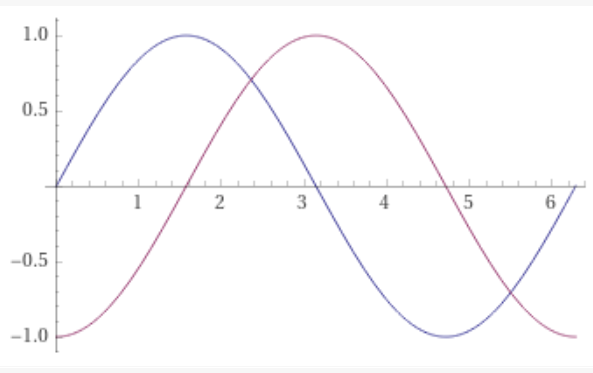
\includegraphics[width=0.9\textwidth]{05/phaseshift.png}};
\node at (-1.6,2.0) { \textcolor{blue}{not reflected}};
\node at (1.7,2.0)  { \textcolor{purple}{reflected}};
\end{TIKZP}
\begin{center}
{\small Thanks to Rick Roesler for this plot}
\end{center}
}
}{%
\Vskip{-4em}\begin{center}
\begin{TIKZP}[scale=2.0]
    \draw[thick,color=red] (0,0.5) -- ++(0.5,0);
    \visible<1,4->{\draw[->,thick,color=red] (0,0.5) -- ++(0.5,0) -- ++(0,-0.5);}
    \visible<1-3>{\draw[->,thick,color=red] (0.5,0.5) -- (1.0,0.5);}
    \visible<1-2,4->{\RotateAroundCenter{-45}{\BeamSplitter{}}}
\end{TIKZP}
\end{center}
\visible<5->{%
When reflected, we assume here that the photon experiences \textcolor<6->{purple}{a delay of $\frac{\pi}{2}$ radians} compared with \textcolor<6->{blue}{one passing through the beam splitter}.
}
}

\end{frame}

\begin{frame}{Analysis of the photon's paths}{A demonstration of interference}

\Vskip{-4em}\TwoUnequalColumns{0.55\textwidth}{0.45\textwidth}{%
\begin{itemize}
  \item<1-> A photon is measured \textcolor{NavyBlue}{here} using one of two paths:
  \begin{itemize}
      \item<2-> \textcolor{purple}{Here, the photon is reflected by a mirror, but passes through both beam splitters.  \alert<2>{There is no phase shift in this case.}}
      \item<3-> \textcolor{OliveGreen}{Here, the photon is reflected by each beam splitter.  \alert<3>{The accumulated delay is therefore $2\times \pi/2 = \pi$~radians.}}
  \end{itemize}
  \item<4-> \textcolor{NavyBlue}{Where the paths converge, the waves cancel, so there is no probability of measurement here.}
  \item<5> \textcolor{orange}{All photons are measured here.}
\end{itemize}
}{%
\Vskip{-2em}
\begin{center}
\begin{TIKZP}[scale=0.655]
\MZ{}
\draw[color=red] (1,0.5) -- (2.5,0.5);
\draw[color=purple] (2.5,0.5) -- ++(4,0) -- ++(0,-2);
\draw<2>[ultra thick,color=purple] (2.5,0.5) -- ++(4,0) -- ++(0,-3.5);
\draw[color=OliveGreen] (2.5,0.5) -- ++(0,-2) -- ++(4,0);
\draw<3>[ultra thick,color=OliveGreen] (2.5,0.5) -- ++(0,-2) -- ++(4,0) -- ++(0,-1.5);
\draw<1,5->[->,color=orange] (6.5,-1.5) -- ++(1.5,0);
\draw<1-4>[->,color=NavyBlue] (6.5,-1.5) -- ++(0,-1.5);
\end{TIKZP}
\MedSkip{}

\only<1-4>{
\begin{TIKZP}
\visible<2,4>{
\begin{scope}[color=purple]
\SineWave{1.0}
\end{scope}}
\visible<3,4>{
\begin{scope}[color=OliveGreen]
\SineWave{-1.0}
\end{scope}}
\end{TIKZP}}
\end{center}
\only<5->{
Physics experiments have confirmed this behavior.
We will soon look at how to model this behavior mathematically.}
}
\end{frame}

\begin{frame}{The quantum eraser}{This material can be skipped, but you may find it interesting.}
\begin{itemize}
    \item A \href{https://www.scientificamerican.com/article/slide-show-do-it-yourself-diy-quantum-eraser/}{do-it yourself} approach.
    \item This material from \href{https://www.physlab.org/wp-content/uploads/2016/07/machzehnder-v4.pdf}{here}
    \item PBS Space Time: \href{https://www.youtube.com/watch?v=8ORLN_KwAgs}{How the Quantum Eraser Rewrites the Past}
    \item PBS Space Time: \href{https://www.youtube.com/watch?v=2Uzytrooz44}{Quantum Eraser Lottery Challenge}
\end{itemize}
\end{frame}

\begin{frame}{Accounting for a phase shift of $\pi/2$ radians}{We use complex numbers.}
\Vskip{-3em}\TwoUnequalColumns{0.7\textwidth}{0.3\textwidth}{%
\begin{itemize}
    \item Recall the complex unit circle.  
    \item Suppose we begin with an amplitude $\alpha$, which already has an arbitrary phase shift.
    \item<2-> $\ExpPhase{0}\alpha = 1\times \alpha$ represents no (further) phase shift.
    \item<3-> The shift of $\alpha$ by $\theta$ radians is then $\ExpPhase{\theta}\alpha$.
   
    
\end{itemize}
}{%
\begin{center}
    \begin{TIKZP}
        \UnitComplexCircle{}
        \visible<4->{\TZPNorth{}
        \draw[->,ultra thick] (0,0) -- (0,1);}
        \visible<2->{\TZPEast{}}
        \visible<3>{\draw[->,thick] (1,0) arc (0:45:1) coordinate (z) ;
    \draw[thick] (0,0) -- (z) ;
    \draw (0.3,0) node[above right] {$\theta$};}
        \visible<4->{\TZPSouth{}
        \TZPWest{}}
    \end{TIKZP}
\end{center}
}
\OnlyRemark{4}{The shift of an amplitude by $\pi/2$ radians is effected through multiplication by $\ExpPhase{\pi/2} = i$.}
\end{frame}
\begin{frame}{Properties of phase shifts}{Complex math helps here too.}
\Vskip{-3em}\TwoUnequalColumns{0.7\textwidth}{0.3\textwidth}{%
\begin{itemize}
    \item<1-> A phase shift has no effect on the wave's magnitude:
    \[
    \Forall{\theta}{%
    \Mag{\ExpPhase{\theta}\alpha} = \Mag{\ExpPhase{\theta}} \times \Mag{\alpha} 
    = 1 \times \Mag{\alpha} = \Mag{\alpha}
    }
    \]
    \item<2-> A shift of $\alpha$ by $\theta$ radians followed
    by a shift of $\phi$ radians is given by
    \[
       \ExpPhase{\phi}\left(\ExpPhase{\theta}\alpha\right) = \ExpPhase{(\theta+\phi)}\alpha
    \]
    which walks counter-clockwise around the unit circle $\theta$ and then $\phi$ radians.
\end{itemize}
}{%
\begin{center}
    \begin{TIKZP}
        \UnitComplexCircle{}
        \TZPNorth{}\TZPSouth{}\TZPEast{}\TZPWest{}
        \visible<1->{
            \draw[->,thick] (1,0) arc (0:45:1) coordinate (z) ;
            \draw[thick] (0,0) -- (z) ;
            \draw (0.3,0) node[above right] {$\theta$};
        }
        \visible<2->{
            \draw[->,thick] (1,0) arc (0:135:1) coordinate (z) ;
            \draw[thick] (0,0) -- (z) ;
            \draw (0,0.2) node[above left] {$\phi$};
        }
    \end{TIKZP}
\end{center}
}
\end{frame}

\begin{frame}{Creating an equal superposition}{We can determine much about the amplitude from the desired probability.}
\Vskip{-3em}\TwoUnequalColumns{0.6\textwidth}{0.4\textwidth}{%
\begin{itemize}
    \item<1-> We begin with a ground state such as \ket{0}.
    \item<2-> From \ket{0}, we wish to create an equal superposition of \ket{0} and \ket{1}.
    \item<3-> That is, we want the probability of measuring either outcome to be $\frac{1}{2}$.
    \item<4-> From this we know the magnitude of the associated wave amplitudes must be $\frac{1}{\sqrt{2}}$.
    \item<5-> We are thus seeking the state
    \[ \alpha\ket{0} + \beta\ket{1} \]
    subject to $\Mag{\alpha} = \Mag{\beta} = \frac{1}{\sqrt{2}}$
\end{itemize}
}{%
\Vskip{-4em}\begin{center}
\begin{TIKZP}[scale=2.0]
    \draw[thick,color=red] (0,0.5) -- ++(0.5,0);
    \visible<1->{\draw[->,thick,color=red] (0,0.5) -- ++(0.5,0) -- ++(0,-0.5);}
    \visible<1->{\draw[->,thick,color=red] (0.5,0.5) -- (1.0,0.5);}
    \visible<1->{\RotateAroundCenter{-45}{\BeamSplitter{}}}
\end{TIKZP}
\end{center}
\visible<6->{
\BigSkip{}
Each wave amplitude must therefore be of the form
\[\frac{1}{\sqrt{2}}\ExpPhase{\theta} \]
}
}
\end{frame}
\def\BSG{%
\ensuremath{\frac{1}{\sqrt{2}}
\begin{pmatrix}
1 & i \\
i & 1
\end{pmatrix}}}

\section{Quantum gates}

\begin{frame}{Modeling the beam splitter}{Our first quantum gate}

\def\ralpha{\ensuremath{\textcolor{red}{\alpha}}}
\def\bbeta{\ensuremath{\textcolor{brown}{\beta}}}
\def\ralphap{\ensuremath{\textcolor{orange}{\alpha'}}}
\def\bbetap{\ensuremath{\textcolor{NavyBlue}{\beta'}}}


\Vskip{-3em}\TwoUnequalColumns{0.5\textwidth}{0.5\textwidth}{%
\visible<1->{Suppose the beam splitter is presented with a photon in superposition
    \[\ket{\psi}=
    \visible<1->{\ralpha\textcolor{red}{\ket{0}}}
    \visible<2->{+ \bbeta\textcolor{brown}{\ket{1}}
    = \SQB{\ralpha}{\bbeta}
    }
    \]}
    \visible<5->{%
    \Vskip{-1.5em}The output is then
    \begin{eqnarray*}
     \ket{\psi'} & = & \SQB{\ralphap{}}{\bbetap{}} \\
     \ralphap{} & = & \frac{1}{\sqrt{2}}\left(\visible<6->{\ralpha{}}
        + \visible<7->{i\bbeta{}}\right) \\
    \visible<8->{\bbetap{} & = & \frac{1}{\sqrt{2}}\left(\visible<9->{i\ralpha{}}
         + \visible<10->{\bbeta{}}\right)}
    \end{eqnarray*}}
}{%
\only<1-10>{%
\Vskip{-4em}
\begin{center}
\begin{TIKZP}[scale=2.5]
    \visible<1->{\RotateAroundCenter{-45}{\BeamSplitter{}}}
    \visible<1->{\draw[->,color=red] (0,0.5) node[left] {$\alpha$}  -- node[midway,below]  {\ket{0}} ++(0.5,0);}
    \visible<2->{\draw[->,color=brown] (0.5,1) node[above] {$\beta$} -- node[midway,right] {\ket{1}} ++(0, -0.5);}
    \visible<3->{\draw[->,color=orange] (0.5,0.5) -- (1.0,0.5) node[right] {$\alpha'$};}
    \visible<4->{\draw[->,color=NavyBlue] (0.5,0.5) -- ++(0,-0.5) node[below] {$\beta'$};}
    
\end{TIKZP}
\end{center}
\only<3-4>{We want to compute the effect of the beam splitter in creating a superposition of outputs: \textcolor{orange}{photon traveling east} and \visible<4->{\textcolor{NavyBlue}{photon traveling south}}}
\only<5-7>{\ralphap{} is composed of an equal fraction of \only<6-7>{\ralpha{} continuing right} \only<7>{and \bbeta{} reflecting to the right with a $\frac{\pi}{2}$ phase shift.}}
\only<8-10>{\bbetap{} is composed of an equal fraction of \only<9-10>{\ralpha{} reflecting down with a $\frac{\pi}{2}$ phase shift} \only<10>{and \bbeta{} continuing down.}}
}%
\only<11->{%
We can model the effect of the beam splitter using the following matrix algebra:
\[
\SQB{\ralphap{}}{\bbetap{}} = 
\BSG{} \SQB{\ralpha}{\bbeta}
\]
and we view the beam splitter as represented mathematically as
\[
\BSG{}
\]
}
}
\end{frame}

\begin{frame}{Applying the beam splitter to our example}{Matrix multiplication models the cumulative effect of gates.}

\TwoUnequalColumns{0.6\textwidth}{0.4\textwidth}{%
\Vskip{-2em}\begin{itemize}
    \only<1-2>{
    \item We begin with the photon in state \SQB{1}{0}.}
    \only<2-3>{\item At the first beam splitter, we obtain the state
    \[ \BSG{} \SQB{1}{0} = \frac{1}{\sqrt{2}} \SQB{1}{i}
    \]}
    \only<3-4>{\item The mirrors flip the sense of two paths with respect to the second beam splitter.  We therefore apply a gate to swap the two components and obtain
    \[
    \XMatrix{} \RootTwo{}\SQB{1}{i} = \RootTwo{}\SQB{i}{1}
    \]}
    \only<4-5>{\item The final beam splitter produces
    \[
    \BSG{}\RootTwo{}\SQB{i}{1} = \frac{1}{2}\SQB{2i}{i^{2}+1} = \SQB{i}{0}
    \]}
    \only<5>{\item The interference canceled the bottom component.    
    \alert{This explains why the bottom device never measures any photons in this setup.}
    \item
    We can also see the top component is rotated by $\pi/2$ radians.  The superpositions measured \textcolor{orange}{by this device} each experienced one beam-splitter reflection.}
\end{itemize}
}{%
\begin{center}
    \Vskip{-3em}\begin{TIKZP}[scale=0.5]
        \MZ{}
        \visible<2>{\Shift{2}{0}{\RotateAroundCenter{-45}{\BeamSplitter[ultra thick]{}}}}
        \visible<4>{\Shift{6}{-2}{\RotateAroundCenter{-45}{\BeamSplitter[ultra thick]{}}}}
        \draw[color=red] (1,0.5) -- (2.5,0.5);
        \draw<1>[ultra thick,color=red] (1,0.5) -- (2.5,0.5);
        \draw[color=purple] (2.5,0.5) -- ++(4,0) -- ++(0,-2);
        \draw[color=OliveGreen] (2.5,0.5) -- ++(0,-2) -- ++(4,0);
        \draw[->,color=orange] (6.5,-1.5) -- ++(1.5,0);
        \draw[->,color=NavyBlue] (6.5,-1.5) -- ++(0,-1.5);
    \end{TIKZP}
    \begin{TIKZP}[scale=1.5]
    \visible<1->{\RotateAroundCenter{-45}{\BeamSplitter{}}}
    \visible<1->{\draw[->,color=red] (0,0.5) node[left] {$\alpha$}  -- node[midway,below]  {\ket{0}} ++(0.5,0);}
    \visible<1->{\draw[->,color=brown] (0.5,1) node[above] {$\beta$} -- node[midway,right] {\ket{1}} ++(0, -0.5);}
    \visible<1->{\draw[->,color=orange] (0.5,0.5) -- (1.0,0.5) node[right] {$\alpha'$};}
    \visible<1->{\draw[->,color=NavyBlue] (0.5,0.5) -- ++(0,-0.5) node[below] {$\beta'$};}
    
\end{TIKZP}
\end{center}
}
    
\end{frame}

\begin{frame}{Quantum gates as matrices}{What properties must they have?}

\begin{itemize}
    \item Recall that the quantum state of a single qubit can be represented by the ket
    $\SQB{\alpha}{\beta}$, where $\alpha$ and $\beta$ are complex numbers.  We require $\Prob{\alpha}+\Prob{\beta}=1$.  Such vectors are called \href{https://en.wikipedia.org/wiki/Unit_vector}{unit vectors}.
    \item A matrix can represent the action of a quantum gate, but it must have the following properties:
    \begin{itemize}
        \item It must be \href{https://en.wikipedia.org/wiki/Reversible_computing}{reversible}. We have already studied this property.
        \item It must be \emph{length-preserving}.  If $U$ is such a matrix, then $\Implies{\Mag{\alpha}=1}{\Mag{U\alpha}=1}$. Informally, no \Quote{probability} is gained or lost by application of $U$.
    \end{itemize}
     
\end{itemize}
    The matrices we seek are \href{https://en.wikipedia.org/wiki/Unitary_matrix}{unitary}.   We next investigate their definition and properties.
\end{frame}

\begin{frame}{Unitary matrix}{Definition and properties \LinkArrow{https://en.wikipedia.org/wiki/Unitary_matrix}}

\Definition{%
The matrix $U$ is \emph{unitary} iff $U\Conj{U}=\Conj{U}U=\Identity$}
\begin{center}Equivalent conditions\end{center}

\TwoColumns{%

\begin{itemize}
    \item $U$ is unitary
    \item \Conj{U} is unitary
    \item $U$ is invertible with $\Inverse{U}=\Conj{U}$
    \item The columns of $U$ form an \href{https://en.wikipedia.org/wiki/Orthonormal_basis}{orthonormal basis}; so do the rows.
\end{itemize}
}{%
\begin{itemize}
    \item $U$ is a \href{https://en.wikipedia.org/wiki/Normal_matrix}{normal matrix} whose eigenvalues lie on the (real) unit circle.
\end{itemize}
}

\end{frame}

\section{Summary}
\begin{frame}{Summary}{What have we learned?}
\begin{itemize}
    \item A quantum state is represented by a column vector called a \emph{ket}.  The \href{https://en.wikipedia.org/wiki/Qubit\#Standard_representation}{standard computational basis} for a single qubit uses $\ket{0}=\PZero{}$ and $\ket{1}=\POne{}$.
    \item Superpositions are expressed as linear combinations of basis states.  
    \item The wave amplitude on each basis state is a complex number, which expresses both magnitude and phase.
    \item We model a quantum gate using a unitary matrix.  For a single qubit, such matrices are $2\times 2$.
    \item The effect of a gate on a quantum state is computed using matrix multiplication.
\end{itemize}
    
\end{frame}
\frame{Assignment ps1}
\frame{Programming assignment q0}

\end{document}
